%%%%%%%%%%%%%%%%%%%%%%%%%%%%%%%%%%%%%%%%%
% University/School Laboratory Report
% LaTeX Template
% Version 3.1 (25/3/14)
%
% This template has been downloaded from:
% http://www.LaTeXTemplates.com
%
% Original author:
% Linux and Unix Users Group at Virginia Tech Wiki 
% (https://vtluug.org/wiki/Example_LaTeX_chem_lab_report)
%
% License:
% CC BY-NC-SA 3.0 (http://creativecommons.org/licenses/by-nc-sa/3.0/)
%
%%%%%%%%%%%%%%%%%%%%%%%%%%%%%%%%%%%%%%%%%

%----------------------------------------------------------------------------------------
%	PACKAGES AND DOCUMENT CONFIGURATIONS
%----------------------------------------------------------------------------------------

\documentclass{article}

%\usepackage[version=3]{mhchem} % Package for chemical equation typesetting
%\usepackage{siunitx} % Provides the \SI{}{} and \si{} command for typesetting SI units
\usepackage{graphicx} % Required for the inclusion of images
\usepackage{natbib} % Required to change bibliography style to APA
\usepackage{amsmath} % Required for some math elements 
\usepackage[left=3cm,top=3cm,right=3cm,bottom=3cm]{geometry} %%Márgenes
\usepackage[section]{placeins}
% Paquetes a usar
\usepackage[english]{babel}   %%para Colocar el Espa\~{u}ol
\usepackage[utf8]{inputenc} %%para usar tildes adecuadamente
\usepackage{amssymb}          % S\'{i}mbolos
\usepackage{hyperref}         % Vinculos 
\usepackage{graphics}         % Subfiguras
\usepackage{pdfpages}         % incluir PDF
\usepackage[tight,footnotesize]{subfigure}
%\usepackage{babel}   %%para Colocar el Espa\~{u}ol
\usepackage{pgfplots}

\renewcommand{\contentsname}{Tabla de contenido}
\renewcommand{\partname}{Parte}
\renewcommand{\appendixname}{Ap\'{e}ndice}
\renewcommand{\bibname}{Referencias}
\renewcommand{\figurename}{Figura}
\renewcommand{\listfigurename}{\'{i}ndice de figuras}
\renewcommand{\tablename}{Tabla}
\renewcommand{\listtablename}{\'{i}ndice de tablas}

\let\cleardoublepage\clearpage %Quitar paginas en blanco
\setlength{\parindent}{0pt} % Quitar sangria del inici de parrafo


\setlength\parindent{0pt} % Removes all indentation from paragraphs

\renewcommand{\labelenumi}{\alph{enumi}.} % Make numbering in the enumerate environment by letter rather than number (e.g. section 6)

%\usepackage{times} % Uncomment to use the Times New Roman font

%----------------------------------------------------------------------------------------
%	DOCUMENT INFORMATION
%----------------------------------------------------------------------------------------

\title{Im\'{a}genes y Visi\'{o}n - Taller 6 B: Taller pr\'{a}ctico de procesamiento de im\'{a}genes: Operadores b\'{a}sicos de la morfolog\'{i}a matem\'{a}tica} % Title

\author{
  Jos\'{e} Francisco Molano Pulido\\
  \texttt{jf.molano1587@uniandes.edu.co}
  \and
  Sergio Daniel Hern\'{a}ndez Charpak\\
  \texttt{sd.hernandez204@uniandes.edu.co}
}

\date{\today} % Date for the report

%\pgfplotsset{compat=1.13} 
\begin{document}

\maketitle % Insert the title, author and date

\tableofcontents
% If you wish to include an abstract, uncomment the lines below
% \begin{abstract}
% Abstract text
% \end{abstract}

\newpage
%----------------------------------------------------------------------------------------
%	Etiquetado de objetos - Francisco
%----------------------------------------------------------------------------------------
\section{Etiquetado de objetos}

En esta secci\'{o}n se presentan los resultados del etiquetamiento de objetos aplicado sobre la imagen sic.png (figura \ref{fg:original}).

\begin{figure}[ht]
\begin{center}
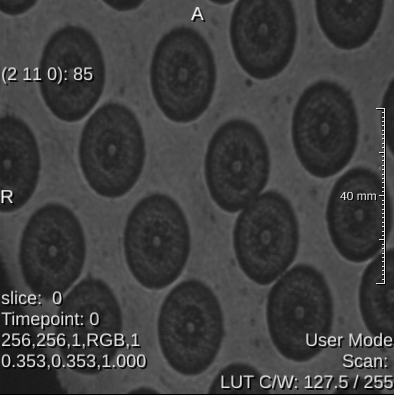
\includegraphics[width=0.37\textwidth]{1Etiquetado/1_img1} % Include the image placeholder.png
\caption{Imagen sic.png original}
\label{fg:original}
\end{center}
\end{figure}
\FloatBarrier

En primer lugar, se aplica una umbralizaci\'{o}n sobre la imagen original para obtener una primera aproximaci\'{o}n a la separaci\'{o}n de las estructuras, en este caso las c\'{e}lulas. El resultado es presentado en la figura \ref{fg:segmentada}.

\begin{figure}[ht]
\begin{center}
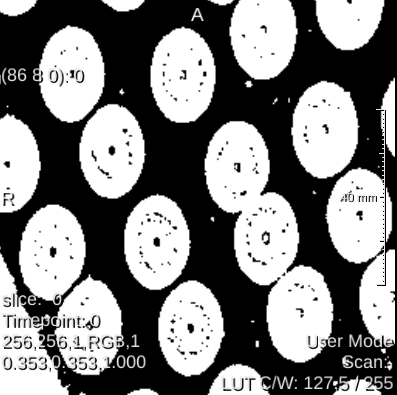
\includegraphics[width=0.37\textwidth]{1Etiquetado/1_img2} % Include the image placeholder.png
\caption{Resultado de umbralizaci\'{o}n de la imagen sic.png (valor de umbral = 60)}
\label{fg:segmentada}
\end{center}
\end{figure}
\FloatBarrier

En la imagen resultante presentada en la figura \ref{fg:segmentada} se observa que el umbral aplicado permiti\'{o} una separaci\'{o}n aceptable de las estructuras y el fondo. Sin embargo, las c\'{e}lulas identificadas aun presentan huecos y algunas de ellas se encuentran unidas, este factor impide realizar un proceso de conteo autom\'{a}tico. Por lo tanto, los siguientes pasos realizados se enfocaron en la correcci\'{o}n de dichos aspectos. En primer lugar, se aplica un proceso de dilataci\'{o}n con el prop\'{o}sito de rellenar los huecos en las estructuras. Los resultados son presentados en la figura \ref{fg:dilatacion}.

\begin{figure}[ht]
\begin{center}
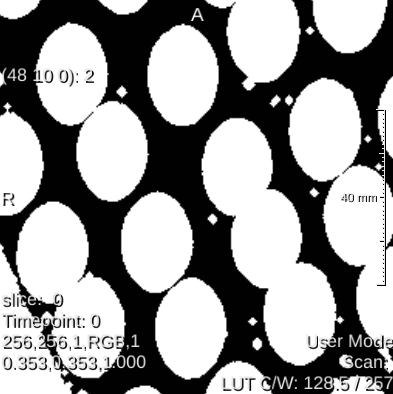
\includegraphics[width=0.37\textwidth]{1Etiquetado/1_img3} % Include the image placeholder.png
\caption{Resultado de dilataci\'{o}n de la imagen en figura \ref{fg:segmentada} (m\'{a}scara en cruz 3x3)}
\label{fg:dilatacion}
\end{center}
\end{figure}
\FloatBarrier

En la figura \ref{fg:dilatacion} se observa que el proceso de dilataci\'{o}n aplicado efectivamente permiti\'{o} realizar una correcci\'{o}n efectiva de los huecos en la imagen, sin embargo se observa un incremento del tama\~{u}o de estructuras secundarias que no corresponden a c\'{e}lulas. Adicionalmente, se observa un incremento en la uni\'{o}n de las estructuras identificadas. Por este motivo, se emplea un proceso de erosi\'{o}n, empleando una m\'{a}scara oblicua. Los resultados son presentados en la figura \ref{fg:erosion}.

\begin{figure}[ht]
\begin{center}
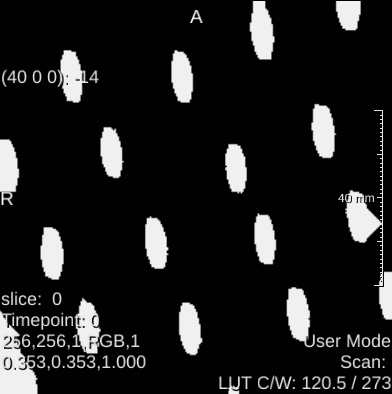
\includegraphics[width=0.37\textwidth]{1Etiquetado/1_img4} % Include the image placeholder.png
\caption{Resultado de erosi\'{o}n de la imagen en figura \ref{fg:dilatacion} (m\'{a}scara oblicua 3x3)}
\label{fg:erosion}
\end{center}
\end{figure}
\FloatBarrier

Al observar el resultado de las erosiones aplicadas (figura \ref{fg:erosion}), se afirma que se consigui\'{o} el prop\'{o}sito de separar las distintas c\'{e}lulas en la imagen. A pesar de que las estructuras sufrieron una distorsi\'{o}n notable debido a la operaci\'{o}n de morfolog\'{i}a, el resultado obtenido es suficiente para aplicar el proceso de etiquetamiento y definici\'{o}n del n\'{u}mero de c\'{e}lulas. Adicionalmente, se observa que las estructuras menores que no correspond\'{i}an a c\'{e}lulas en la imagen fueron eliminadas satisfactoriamente. De esta manera, se procede a realizar el proceso de etiquetamiento. Los resultados obtenidos son presentados en la figura \ref{fg:etiquetas}.

\begin{figure}[ht]
\begin{center}
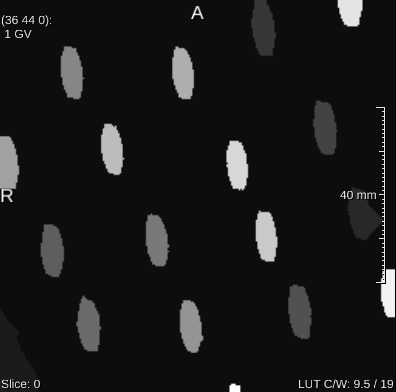
\includegraphics[width=0.37\textwidth]{1Etiquetado/1_img5} % Include the image placeholder.png
\caption{Resultado de etiquetamiento sobre la imagen en figura \ref{fg:erosion}}
\label{fg:etiquetas}
\end{center}
\end{figure}
\FloatBarrier

En la figura \ref{fg:etiquetas} se observa el resultado del proceso de etiquetamiento. En este caso, el algoritmo asigna un valor de intensidad distinto a los p\'{i}xeles correspondientes a cada uno de los objetos identificados (al fondo de la imagen le es asignado un valor de 0). Finalmente, se realiza un an\'{a}lisis de histograma sobre el resultado obtenido con la finalidad de facilitar el proceso de conteo de las c\'{e}lulas. El resultado es presentado en la figura \ref{fg:histograma}.

\begin{figure}[ht]
\begin{center}
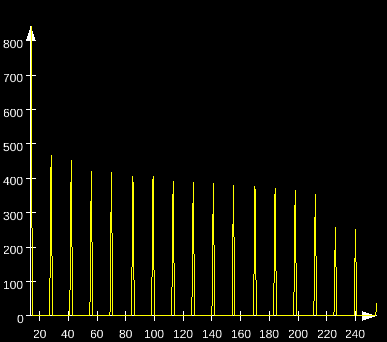
\includegraphics[width=0.37\textwidth]{1Etiquetado/1_img6} % Include the image placeholder.png
\caption{Histograma de la imagen en figura \ref{fg:etiquetas}}
\label{fg:histograma}
\end{center}
\end{figure}
\FloatBarrier

En la figura \ref{fg:histograma} se observa el histograma de la imagen obtenida en el proceso de etiquetamiento, luego de aplicar una calibraci\'{o}n de las intensidades. En este caso se excluye la tonalidad correspondiente al fondo (0) para facilitar el an\'{a}lisis. A partir de la distribuci\'{o}n observada es posible realizar el conteo de estructuras identificadas. En este caso, se etiquetaron 18 c\'{e}lulas. Se debe destacar que mediante este an\'{a}lisis tambi\'{e}n es posible realizar un estudio m\'{a}s detallado de las estructuras. Por ejemplo, es posible determinar, para cada c\'{e}lula, la proporci\'{o}n del tama\~{u}o respecto a la imagen y a las dem\'{a}s estructuras.\\
A pesar de que este m\'{e}todo result\'{o} efectivo identificar las c\'{e}lulas en la imagen, se puede observar que hubo una p\'{e}rdida leve de informaci\'{o}n al aplicar la serie de erosiones, principalmente en los bordes de la imagen. En particular, se perdi\'{o} la informaci\'{o}n correspondiente a seis c\'{e}lulas. Tambi\'{e}n se destaca que en el resultado hay una distorsi\'{o}n notable en la forma del borde de las c\'{e}lulas respecto a la imagen original.



%----------------------------------------------------------------------------------------
%	Imagen de distancia - Sergio
%----------------------------------------------------------------------------------------

\section{Imagen de distancia}

\begin{par}
El objetivo de este punto es de obtener una imagen de distancia. El ejercicio se realiza sobre la imagen \ref{fg:2_orig}.
\end{par}

\begin{figure}[ht]
\begin{center}
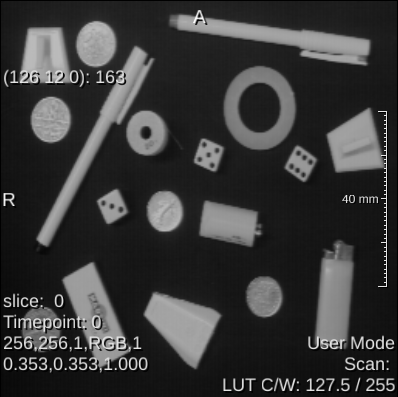
\includegraphics[width=0.37\textwidth]{2Distancia/2_orig} % Include the image placeholder.png
\caption{Imagen Objects original}
\label{fg:2_orig}
\end{center}
\end{figure}
\FloatBarrier

\begin{par}
Primero que todo se debe pasar est\'{a} imagen desde una imagen RGB a una imagen en escala de niveles de gris. Para ellos usamos el m\'{o}dulo ColorModelConverter (que ser\'{a} muy \'{u}til en los ejercicios de la secci\'{o}n \ref{sec:sintesis}. Luego procedemos a una umbralizaci\'{o}n con umbral 70 y obtenemos los objetos en blanco en la figura \ref{fg:2_umbr}.
\end{par}

\begin{figure}[ht]
\begin{center}
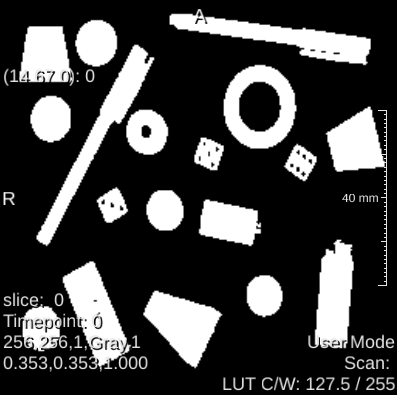
\includegraphics[width=0.37\textwidth]{2Distancia/2_umbr} % Include the image placeholder.png
\caption{Imagen Objects umbralizada}
\label{fg:2_umbr}
\end{center}
\end{figure}
\FloatBarrier

\begin{par}
Una vez umbralizada procedemos a calcular las distancias entre los puntos blancos en la imagen. Por lo tanto los objetos aparecer\'{a}n como negros (al ser blancos, las distancias internas son 0, lo que equivale al negro) y las regiones entre objetos reflejar\'{a}n las distancias entre estos. Podemos observar el resultado efectivo en la figura \ref{fg:2_dist}
\end{par}

\begin{figure}[ht]
\begin{center}
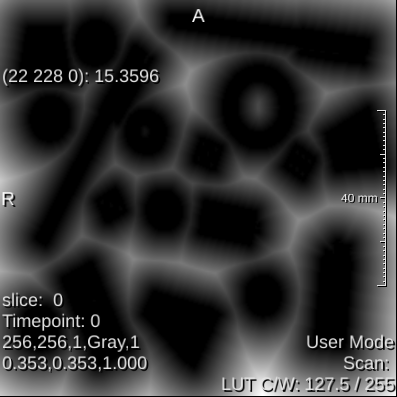
\includegraphics[width=0.37\textwidth]{2Distancia/2_dist} % Include the image placeholder.png
\caption{Distancias entre los objetos, con expansi\'{o}n del contraste para facilitar su observaci\'{o}n}
\label{fg:2_dist}
\end{center}
\end{figure}
\FloatBarrier

\begin{par}
Finalmente calculamos el m\'{a}ximo entre la figura umbralizada \ref{fg:2_umbr} y la imagen de distancia \ref{fg:2_dist} (sin la expansi\'{o}n del contraste). El resultado son los objetos en blanco y en escala de gris (con 0 la distancia m\'{i}nima y 255 la distancia m\'{a}xima) las distancias entre los objetos. Este resultado se puede observar en la figura \ref{fg:2_final}.  
\end{par}

\begin{figure}[ht]
\begin{center}
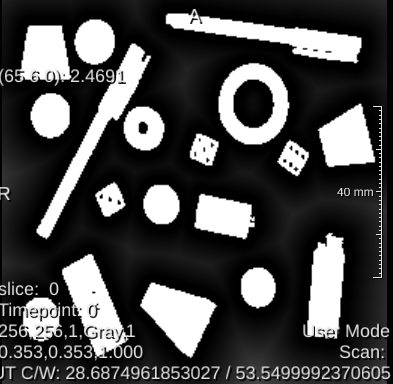
\includegraphics[width=0.37\textwidth]{2Distancia/2_final} % Include the image placeholder.png
\caption{Objetos, con las distancias entre ellos}
\label{fg:2_final}
\end{center}
\end{figure}
\FloatBarrier

\begin{par}
La distancia m\'{i}nima en la figura \ref{fg:2_final} entre los l\'{a}pices equivale entonces al nivel de gris m\'{a}s claro entre ellos en la secci\'{o}n en donde se encuentran m\'{a}s cercanos multiplicado por el tama\~{u}o de un pixel. Este punto se puede observar en la figura \ref{fg:2_min}, sus coordenadas son (102, 24) y su nivel de gris es aproximadamente 4.02. La distancia m\'{i}nima ser\'{a} entonces: $d_{min} (lapiz_1, lapiz_2) = 4.02 size_{pixel} $
\end{par}

\begin{figure}[ht]
\begin{center}
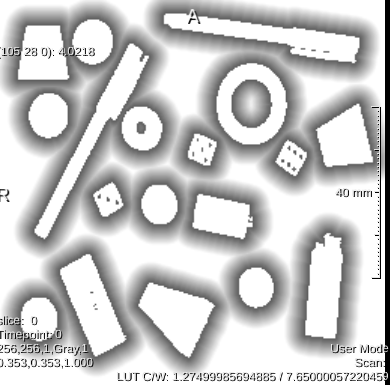
\includegraphics[width=0.37\textwidth]{2Distancia/2_min} % Include the image placeholder.png
\caption{Distancias entre los objetos, los n\'{u}meros en la esquina superior izquierda muestran el punto de distancia m\'{i}nima entre los l\'{a}pices}
\label{fg:2_min}
\end{center}
\end{figure}
\FloatBarrier

%----------------------------------------------------------------------------------------
%	Esqueleto y adelgazamiento de una imagen - Francisco
%----------------------------------------------------------------------------------------

\section{Esqueleto y adelgazamiento de una imagen}

En esta secci\'{o}n se presentan los resultados de aplicar operaciones de esqueletizaci\'{o}n y adelgazamiento sobre im\'{a}genes de prueba. En primer lugar, se realiza el an\'{a}lisis sobre la imagen rect.png (figura \ref{fg:3_original1}) con la finalidad de evaluar el comportamiento de las operaciones mencionadas sobre una imagen b\'{a}sica. 

\begin{figure}[ht]
\begin{center}
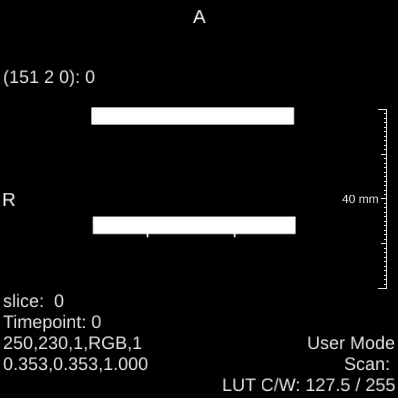
\includegraphics[width=0.37\textwidth]{3Esqueleto/3_original1} % Include the image placeholder.png
\caption{Imagen rect.png original}
\label{fg:3_original1}
\end{center}
\end{figure}
\FloatBarrier

En primer lugar, se aplica la esqueletizaci\'{o}n a la imagen de prueba, los resultados obtenidos son presentados en la figura \ref{fg:esqueleto1}.

\begin{figure}[ht]
\begin{center}
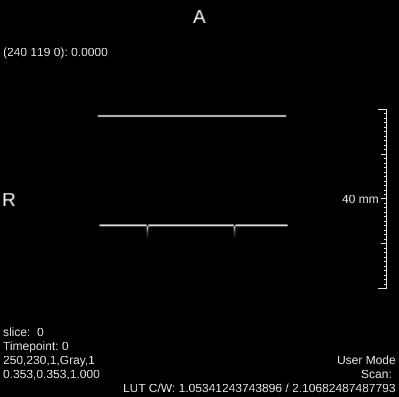
\includegraphics[width=0.37\textwidth]{3Esqueleto/3_skelet1} % Include the image placeholder.png
\caption{Resultado de esqueletizaci\'{o}n en imagen rect.png}
\label{fg:esqueleto1}
\end{center}
\end{figure}
\FloatBarrier

A partir de los resultados obtenidos se observa que la funcionalidad del m\'{o}dulo DtfSkeletonization corresponde a obtener el esqueleto, el cual corresponde a la l\'{i}nea central de un objeto. Esta estructura corresponde al conjunto de puntos que son equidistantes a, por lo menos, dos puntos en la frontera del objeto. Dicho proceso se realiza mediante erosiones sucesivas aplicadas sobre los p\'{i}xeles superficiales del objeto hasta que s\'{o}lo se preserve el esqueleto del mismo. Estas erosiones son aplicadas teniendo en cuenta tres criterios principales:
\begin{itemize}
    \item La erosi\'{o}n de los p\'{i}xeles no debe alterar la topolog\'{i}a de la estructura original. El n\'{u}mero de objetos conectados, cavidades, entre otros, debe permanecer igual.
    \item La erosi\'{o}n debe ser aplicada de forma sim\'{e}trica para garantizar una posici\'{o}n central del esqueleto.
    \item Las superficies ruidosas no deben conllevar a l\'{i}neas de esqueleto irrelevantes que puedan ser interpretadas como ramas del esqueleto principal \cite{esqueleto}.
\end{itemize}
Posteriormente, se realiza el mismo proceso de esqueletizaci\'{o}n pero en este caso, se anula la selecci\'{o}n de la opci\'{o}n Skeleton Only. Los resultados son presentados en la figura \ref{fg:notonly1}.

\begin{figure}[ht]
\begin{center}
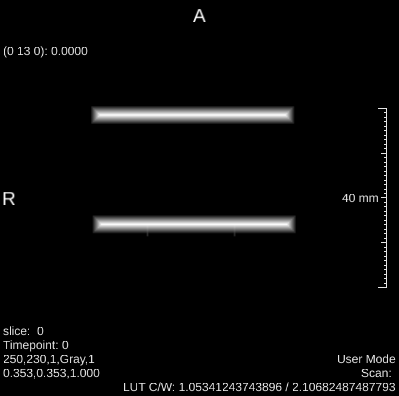
\includegraphics[width=0.37\textwidth]{3Esqueleto/3_skelet_notonly1} % Include the image placeholder.png
\caption{Resultado de esqueletizaci\'{o}n sin opci\'{o}n Skeleton Only en imagen rect.png}
\label{fg:notonly1}
\end{center}
\end{figure}
\FloatBarrier

En la figura \ref{fg:notonly1} se observa que el resultado obtenido no corresponde \'{u}nicamente al esqueleto del objeto en cuesti\'{o}n. En este caso se aprecia la inclusi\'{o}n de niveles adicionales de gris. Seg\'{u}n la documentaci\'{o}n del software MeVisLab, la no selecci\'{o}n de este par\'{a}metro en las opciones del m\'{o}dulo realiza la inclusi\'{o}n de las distancias (en mil\'{i}metros) a la l\'{i}nea central \cite{esqueletoMevis}. Es por este motivo que se observa que las tonalidades m\'{a}s altas est\'{a}n concentradas hacia el esqueleto en cuesti\'{o}n. Luego, se procede a aplicar un adelgazamiento sobre la imagen con el prop\'{o}sito de comparar el desempe\~{u}o de ambas t\'{e}cnicas. Los resultados obtenidos son presentados en la figura \ref{fg:thin1}.

\begin{figure}[ht]
\begin{center}
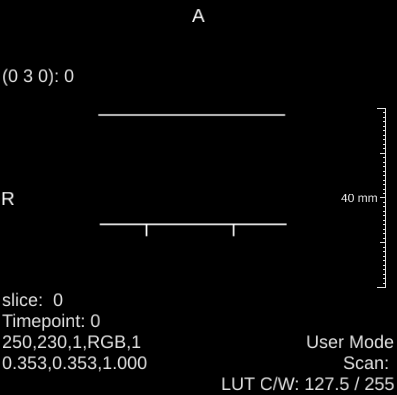
\includegraphics[width=0.37\textwidth]{3Esqueleto/3_thin1} % Include the image placeholder.png
\caption{Resultado de adelgazamiento en imagen rect.png}
\label{fg:thin1}
\end{center}
\end{figure}
\FloatBarrier

En este caso se observa un resultado similar al obtenido mediante esqueletizaci\'{o}n. Sin embargo, se observan diferencias sutiles en las regiones del rect\'{a}ngulo que presentan salidas. En el caso de la esqueletizaci\'{o}n, se observa una l\'{i}nea central con curvaturas. Por otro lado, en el caso del adelgazamiento, se observa un esqueleto con trazos netamente rectos. Adicionalmente, en el caso de la erosi\'{o}n, se obtiene una imagen con distintos niveles de intensidad, dadas por las distancias de erosi\'{o}n medidas en mil\'{i}metros. En el caso del adelgazamiento, se obtiene como resultado una imagen binaria. \\
Una vez concluido el an\'{a}lisis sobre la imagen b\'{a}sica, se procede a aplicar el mismo procedimiento sobre una imagen de mayor complejidad, en este caso, angio.png (figura \ref{fg:3_original2}).

\begin{figure}[ht]
\begin{center}
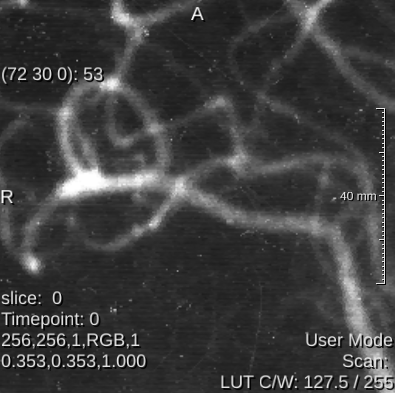
\includegraphics[width=0.37\textwidth]{3Esqueleto/3_original2} % Include the image placeholder.png
\caption{Imagen angio.png original}
\label{fg:3_original2}
\end{center}
\end{figure}
\FloatBarrier

En primer lugar, se realiza una preparaci\'{o}n previa de la imagen. Se realiza una umbralizaci\'{o}n mediante OTSU con el objetivo de realizar una diferenciaci\'{o}n inicial del fondo y el objeto. El resultado es presentado en la figura \ref{fg:otsu2}.

\begin{figure}[ht]
\begin{center}
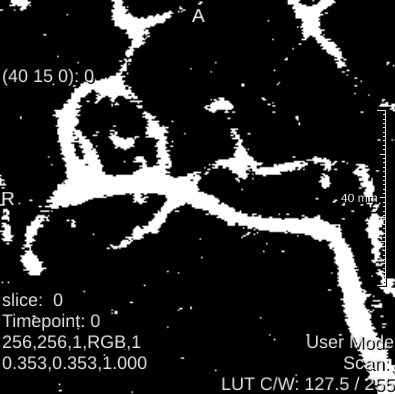
\includegraphics[width=0.37\textwidth]{3Esqueleto/3_otsu2} % Include the image placeholder.png
\caption{Resultado de umbralizaci\'{o}n OTSU sobre angio.png}
\label{fg:otsu2}
\end{center}
\end{figure}
\FloatBarrier

Posteriormente, se procede a aplicar un cierre y una apertura sobre el resultado de la umbralizaci\'{o}n con el prop\'{o}sito de eliminar irregularidades sobre los bordes de la estructura principal y reducir la cantidad de estructuras menores que no corresponden al objeto de inter\'{e}s. Los resultados son presentados en las figuras \ref{fg:cierre2} y \ref{fg:apertura2}, respectivamente.

\begin{figure}[ht]
\begin{center}
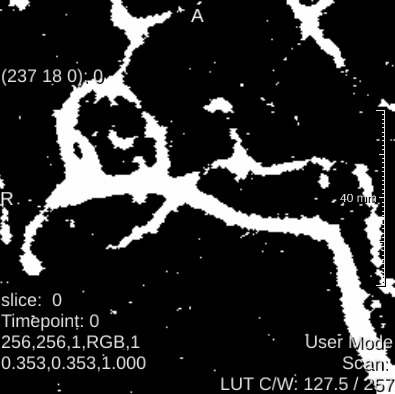
\includegraphics[width=0.37\textwidth]{3Esqueleto/3_cierre2} % Include the image placeholder.png
\caption{Resultado de cierre sobre la imagen umbralizada}
\label{fg:cierre2}
\end{center}
\end{figure}
\FloatBarrier

\begin{figure}[ht]
\begin{center}
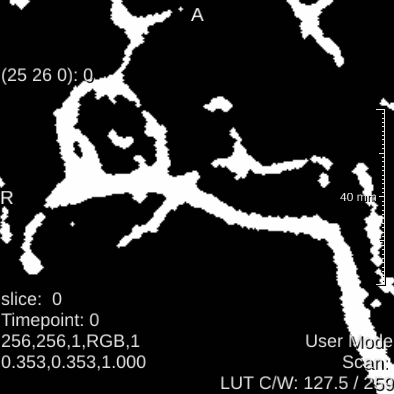
\includegraphics[width=0.37\textwidth]{3Esqueleto/3_apertura2} % Include the image placeholder.png
\caption{Resultado de apertura sobre la imagen sometida al cierre}
\label{fg:apertura2}
\end{center}
\end{figure}
\FloatBarrier

Finalmente, se procede a realizar las operaciones de esqueletizaci\'{o}n (con y sin opci\'{o}n de Skeleton Only) y adelgazamiento. Los resultados son presentados en las figuras \ref{fg:esqueleto2}, \ref{fg:notonly2} y \ref{fg:thin2}, respectivamente.

\begin{figure}[ht]
\begin{center}
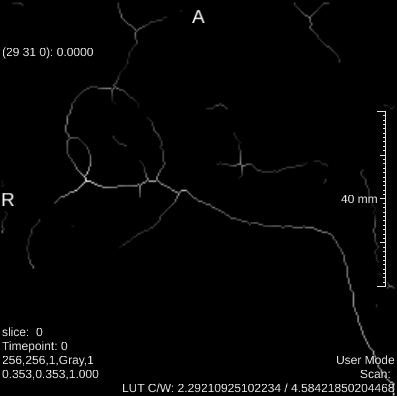
\includegraphics[width=0.37\textwidth]{3Esqueleto/3_skelet2} % Include the image placeholder.png
\caption{Resultado de esqueletizaci\'{o}n con opci\'{o}n Skeleton Only en imagen angio.png procesada}
\label{fg:esqueleto2}
\end{center}
\end{figure}
\FloatBarrier

\begin{figure}[ht]
\begin{center}
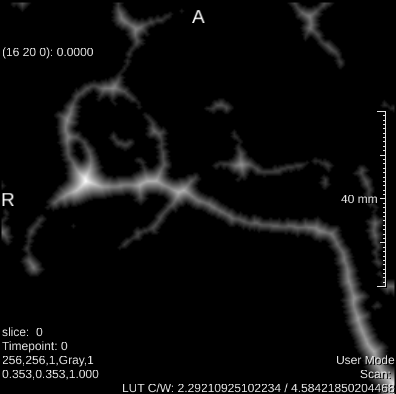
\includegraphics[width=0.37\textwidth]{3Esqueleto/3_skelet_notonly2} % Include the image placeholder.png
\caption{Resultado de esqueletizaci\'{o}n sin opci\'{o}n Skeleton Only en imagen angio.png procesada}
\label{fg:notonly2}
\end{center}
\end{figure}
\FloatBarrier

\begin{figure}[ht]
\begin{center}
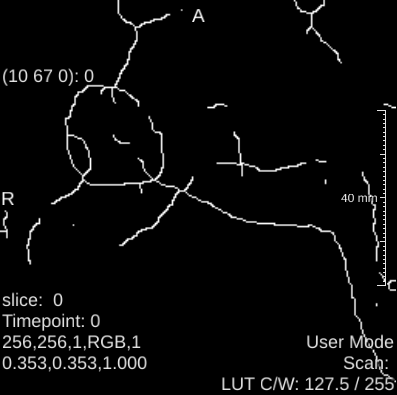
\includegraphics[width=0.37\textwidth]{3Esqueleto/3_thin2} % Include the image placeholder.png
\caption{Resultado de adelgazamiento en imagen angio.png procesada}
\label{fg:thin2}
\end{center}
\end{figure}
\FloatBarrier

Al comparar los resultados de los procesos de esqueletizaci\'{o}n y adelgazamiento, se observa que en general se obtienen productos similares. Sin embargo, tambi\'{e}n es posible apreciar ciertas diferencias. En particular, se observa que el proceso de esqueletizaci\'{o}n tiene como resultado una l\'{i}nea central con trazos m\'{a}s irregulares. El proceso de adelgazamiento presenta trazos m\'{a}s rectos. Adicionalmente, se observa que el proceso de esqueletizaci\'{o}n omite algunos segmentos de la l\'{i}nea central que s\'{i} son incluidos en el resultado del adelgazamiento. Finalmente, se realiza una superposici\'{o}n del resultado obtenido mediante el proceso de adelgazamiento sobre la imagen original, con la finalidad de observar la ubicaci\'{o}n de las l\'{i}neas centrales. Los resultados son presentados en la figura \ref{fg:sobrepuesta}.

\begin{figure}[ht]
\begin{center}
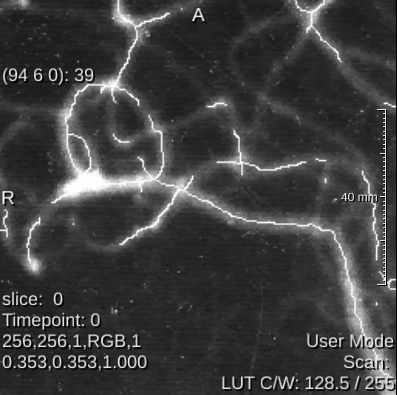
\includegraphics[width=0.37\textwidth]{3Esqueleto/3_sobrepuesta} % Include the image placeholder.png
\caption{Superposici\'{o}n de esqueleto sobre la imagen original angio.png}
\label{fg:sobrepuesta}
\end{center}
\end{figure}
\FloatBarrier

En esta imagen se observa que efectivamente, el algoritmo de adelgazamiento da una buena aproximaci\'{o}n a la l\'{i}nea central del objeto estudiado. Sin embargo, se puede apreciar que en ciertos tramos se presentan discontinuidades en el esqueleto obtenido que no corresponden a la morfolog\'{i}a real de la imagen. Es por este motivo que se sugiere la utilizaci\'{o}n de t\'{e}cnicas m\'{a}s refinadas que permitan realizar la inclusi\'{o}n de los segmentos omitidos.




%----------------------------------------------------------------------------------------
%	Ejercicios de s\'{i}ntesis - Sergio
%----------------------------------------------------------------------------------------

\section{Ejercicios de S\'{i}ntesis}
\label{sec:sintesis}

\subsection{Ejercicio 1}
\begin{par}
El enunciado para este ejercicio es: \textit{Realice las operaciones necesarias
(incluyendo operaciones morfol\'{o}gicas y de segmentaci\'{o}n) sobre la imagen objects.png para
conservar \'{u}nicamente los dos bol\'{i}grafos preservando sus niveles de gris originales (el
resto de la imagen debe quedar negra).}
\end{par}
La imagen a analizar es la siguiente: 

\begin{figure}[ht]
\begin{center}
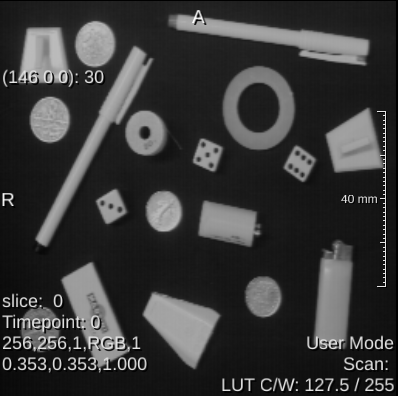
\includegraphics[width=0.4\textwidth]{4Sintesis/4_1_orig} % Include the image placeholder.png
\caption{Imagen Objects original}
\label{fg:4_1_orig}
\end{center}
\end{figure}
\FloatBarrier

\begin{par}
Al estar configurada en RGB es importante que le cambiemos la configuraci\'{o}n a niveles de
grises para que nuestra soluci\'{o}n sea visible.
\end{par}

\begin{par}
Al ser una imagen \ref{fg:4_1_orig} de objetos relativamente uniformes cada uno, podemos
aplicar el m\'{o}dulo (algoritmo) de detecci\'{o}n de regiones por accreci\'{o}n de grupo
directamente sobre esta imagen. Para ello escogemos las semillas en la figura
\ref{fg:4_1_seeds}, dos para ser precisos, una sobre cada uno de los bol\'{i}grafos.
\end{par}

\begin{figure}[ht]
\begin{center}
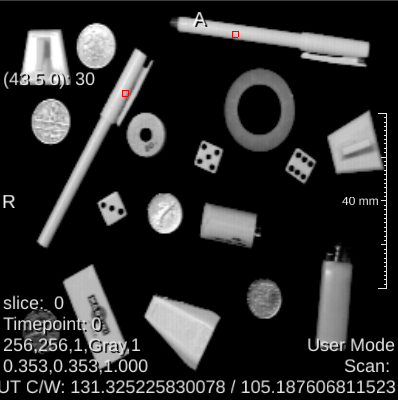
\includegraphics[width=0.4\textwidth]{4Sintesis/4_1_seeds} % Include the image placeholder.png
\caption{Semillas sobre la imagen Objects}
\label{fg:4_1_seeds}
\end{center}
\end{figure}
\FloatBarrier

\begin{par}
Una vez aplicadas las semillas podemos aplicar el m\'{o}dulo (algoritmo) y obtenemos los
resultados deseados en la figura \ref{fg:4_1_objects}. Podemos reconocer nuestros dos
bol\'{i}grafos. Se configur\'{o} el m\'{o}dulo para que los valores de los objetos sean de 255 (valor m\'{a}ximo).
\end{par}

\begin{figure}[ht]
\begin{center}
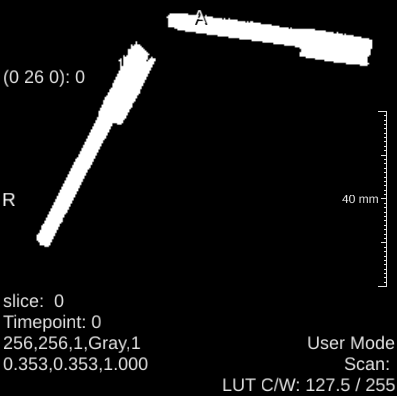
\includegraphics[width=0.4\textwidth]{4Sintesis/4_1_objects} % Include the image placeholder.png
\caption{Objetos detectados sobre la imagen Objects}
\label{fg:4_1_objects}
\end{center}
\end{figure}
\FloatBarrier

\begin{par}
Aplicamos finalmente la operaci\'{o}n AND entre la figura \ref{fg:4_1_objects} de los objetos detectados y la figura original \ref{fg:4_1_orig}. Obtenemos as\'{i} el resultado deseado en la figura \ref{fg:4_1_final}, los dos bol\'{i}grafos con sus valores de niveles de gris originales.
\end{par}

\begin{figure}[ht]
\begin{center}
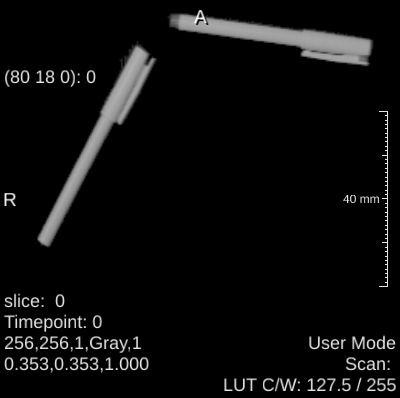
\includegraphics[width=0.4\textwidth]{4Sintesis/4_1_final} % Include the image placeholder.png
\caption{Resultado final, los dos bol\'{i}grafos}
\label{fg:4_1_final}
\end{center}
\end{figure}
\FloatBarrier


\subsection{Ejercicio 3}

\begin{par}
El enunciado para este ejercicio dice: \textit{Realice las operaciones necesarias
(incluyendo operaciones morfol\'{o}gicas y de segmentaci\'{o}n) sobre la imagen meb.png para
conservar \'{u}nicamente las part\'{i}culas peque\~{u}as.}
\end{par}
La imagen a analizar es la siguiente: 

\begin{figure}[ht]
\begin{center}
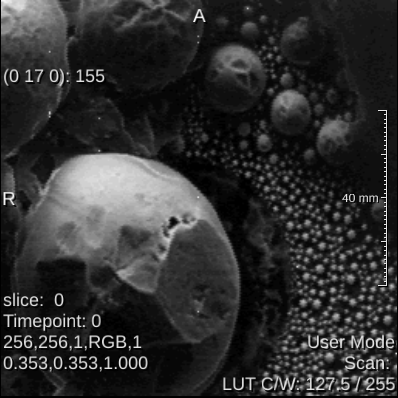
\includegraphics[width=0.4\textwidth]{4Sintesis/4_3_orig} % Include the image placeholder.png
\caption{Imagen Meb original}
\label{fg:4_3_orig}
\end{center}
\end{figure}
\FloatBarrier

\begin{par}
Al no tener objetos relativamente uniformes en la imagen \ref{fg:4_3_orig} y al observar que las part\'{i}culas peque\~{u}as tienen valor de gris relativamente alto la umbralizamos con valor mayor a 100 y obtenemos la figura \ref{fg:4_3_umbr}. 
\end{par}

\begin{figure}[ht]
\begin{center}
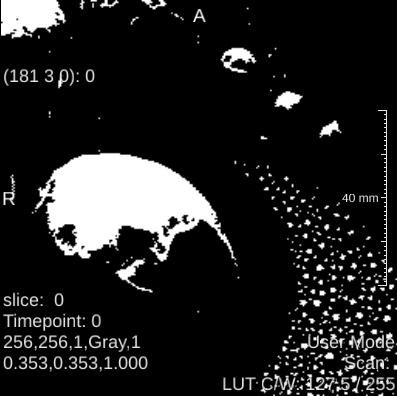
\includegraphics[width=0.4\textwidth]{4Sintesis/4_3_umbr} % Include the image placeholder.png
\caption{Imagen Meb umbralizada}
\label{fg:4_3_umbr}
\end{center}
\end{figure}
\FloatBarrier

\begin{par}
Ya teniendo esta imagen umbralizada \ref{fg:4_3_umbr} escogemos las semillas en las part\'{i}culas grandes en la figura \ref{fg:4_3_seeds}.
\end{par}

\begin{figure}[ht]
\begin{center}
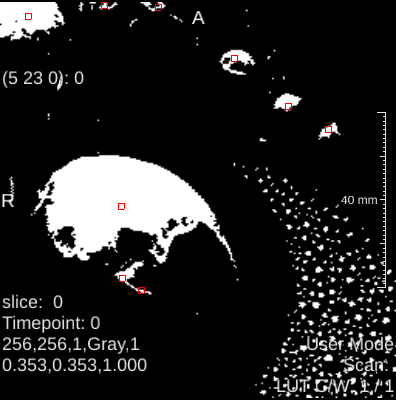
\includegraphics[width=0.4\textwidth]{4Sintesis/4_3_seeds} % Include the image placeholder.png
\caption{Imagen Meb umbralizada con las semillas}
\label{fg:4_3_seeds}
\end{center}
\end{figure}
\FloatBarrier

\begin{par}
Aplicamos as\'{i} el m\'{o}dulo (algoritmo) de detecci\'{o}n de regiones por acreci\'{o}n de grupo y obtenemos as\'{i} los objetos de las part\'{i}culas grandes en la figura \ref{fg:4_3_seeds}.
\end{par}

\begin{figure}[ht]
\begin{center}
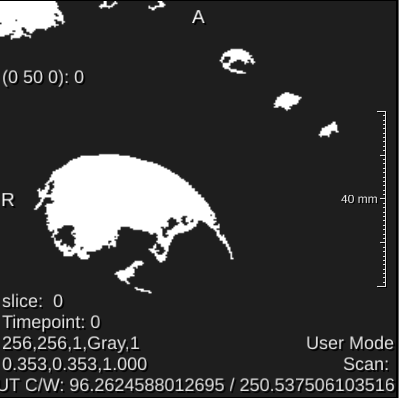
\includegraphics[width=0.4\textwidth]{4Sintesis/4_3_objects} % Include the image placeholder.png
\caption{Objetos detectados Imagen Meb umbralizada}
\label{fg:4_3_objects}
\end{center}
\end{figure}
\FloatBarrier

\begin{par}
Le restamos estos objetos detectados en la figura \ref{fg:4_3_objects} a la imagen
umbralizada \ref{fg:4_3_umbr} y as\'{i} obtenemos el resultado final en la figura
\ref{fg:4_3_final} deseado en donde tenemos las part\'{i}culas peque\~{u}as umbralizadas.
\end{par}

\begin{figure}[ht]
\begin{center}
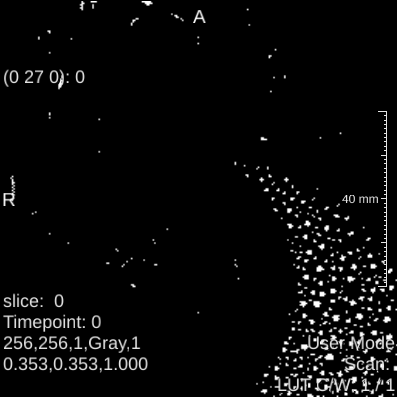
\includegraphics[width=0.4\textwidth]{4Sintesis/4_3_final} % Include the image placeholder.png
\caption{Resultado final, las part\'{i}culas peque\~{u}as}
\label{fg:4_3_final}
\end{center}
\end{figure}
\FloatBarrier

%----------------------------------------------------------------------------------------
%	BIBLIOGRAPHY
%----------------------------------------------------------------------------------------
\nocite{*}
\FloatBarrier

\bibliographystyle{abbrv}

\bibliography{sample}

%----------------------------------------------------------------------------------------

\end{document}
